\documentclass[pre,twocolumn,superscriptaddress,amsmath,amssymb,floatfix]{revtex4-2}
\usepackage{graphicx}
\usepackage{bm}
\usepackage{booktabs}
\usepackage[colorlinks=true,linkcolor=blue,citecolor=blue,urlcolor=blue]{hyperref}

\newcommand{\Sv}{\mathbf{S}}
\newcommand{\qv}{\mathbf{q}}

\begin{document}

\title{Deformable polyhedral spin bodies: multipole channel selection, entropic phase ladders, and non-Abelian orientational order}

\author{Changyeon Won}
\email{cywon@khu.ac.kr}
\affiliation{Department of Physics, Kyung Hee University, Seoul 02447, Republic of Korea}

\date{\today}

\begin{abstract}
We study lattices of ``spin bodies'': clusters of $n$ classical Heisenberg spins that are coupled antiferromagnetically and through higher-order exchange inside each cluster, and ferromagnetically through multi-order exchange between clusters that does not distinguish the spins of a cluster. Inside a cluster the antiferromagnetic exchange enforces a polyhedral arrangement (a regular tetrahedron for $n=4$), so the low-energy object is an orientable polyhedron whose order-parameter space is $SO(3)/T$ with the non-Abelian fundamental group $2T$. Unlike rigid-body models, the polyhedra here are made of spins and can collapse. Decomposing all couplings into multipole channels $l$ we prove that the zero-temperature state is uniform for any lattice, reduce the problem to $n$ particles on a sphere, and obtain exact phase boundaries. Odd channels drive collapse into ferromagnetism and even channels into a collinear nematic, with the ferro--nematic boundary fixed by $z\,g_{\rm odd}(1)=f_{\rm odd}(1)$ for every $n$. A harmonic spin-wave plus configurational (spin-label) free energy then predicts, without fitting parameters, an entropy-driven shift of this boundary, a reentrant ferro-to-nematic transition, and a thin wedge of an equilibrium collinear ferrimagnet between them. Pre-registered Monte Carlo simulations in two and three dimensions confirm the predicted boundary slope $a=0.392\pm0.010$ (theory 0.382--0.390), the reentrance temperature $0.2300\pm0.0026$ (theory $0.234\pm0.008$), and the ferrimagnetic wedge in both dimensions; including the anharmonic free energy by thermodynamic integration reproduces the wedge positions. Transitions with a cubic Landau invariant ($l=2$) are first order, whereas the octupolar ($l=3$) orientational transition of the tetrahedral phase is consistent with a continuous transition up to $L=14$. For $n=6$ the same free energy predicts a four-step ladder; slab coexistence confirms the first collinear step (the M4 phase) and places all boundaries within $0.02$ of the prediction, but does not resolve the M2 phase. We also predict a degenerate prism--octahedron family selected by the ratio of cubic and quartic inter-cluster exchange.
\end{abstract}

\maketitle

%=====================================================================
\section{Introduction}
%=====================================================================

Orientational order of objects with polyhedral symmetry is a recurring theme in condensed matter. Tetrahedral and other polyhedral nematics have been proposed for bent-core liquid crystals~\cite{Fel1995,Lubensky2002}, the cyclic phase of spin-2 Bose--Einstein condensates carries a tetrahedral order parameter with non-Abelian vortices~\cite{SemenoffZhou2007,Kobayashi2009,KawaguchiUeda2012}, and lattice gauge theories have mapped out the generic behavior of nematics with arbitrary point-group symmetry~\cite{Liu2016,Nissinen2016,Liu2017}. In magnetism, noncollinear antiferromagnets are naturally described by cluster multipoles~\cite{Suzuki2017}, multipolar order is central to $f$-electron physics~\cite{Kuramoto2009}, and in breathing pyrochlores strongly bound tetrahedra are weakly coupled to each other~\cite{Okamoto2013,Rau2016}. Molecular solids such as methane realize the quantum version of orientational order of tetrahedral rotors coupled by octupole interactions~\cite{JamesKeenan1959}.

In most of these settings the polyhedron is either rigid by construction (gauge models, molecules) or is a single-site multipole. A different situation arises when the polyhedron is \emph{made of spins}. Then the same exchange that makes the polyhedron also allows it to deform, merge spins, or collapse into a ferromagnet. Two questions follow: Which couplings between such deformable polyhedra stabilize orientational order, and which make the polyhedra collapse? And when competing collapsed states are degenerate in energy, what selects among them at finite temperature?

In this paper we answer both questions for a minimal model, which we call a lattice of spin bodies [Fig.~\ref{fig:model}]. Each body consists of $n$ classical Heisenberg spins with antiferromagnetic (AF) bilinear and biquadratic exchange inside the body, and the bodies are coupled ferromagnetically by cubic and quartic exchange that treats the spins of a body as indistinguishable. Our main findings are:

(i) \emph{Channel selection.} Writing every coupling in Legendre channels $l$, the zero-temperature problem reduces exactly to $n$ particles on a sphere with a pair potential whose spectrum is $\kappa_l=f_l-zg_l$. Odd channels can only produce magnetization and even channels only nematic order. The ferromagnet--nematic boundary is $zg_{\rm odd}(1)=f_{\rm odd}(1)$ for every $n$ and every truncation. In simulations, nematic transition temperatures are independent of the odd-channel coupling, and nematic bodies decouple completely when only odd channels are present.

(ii) \emph{Entropic phase ladder.} Along the ferro--nematic line all collinear states have energies $-\delta M^2/2$ with $\delta=zG-J$, while the number of ways to choose which spins are reversed gives an entropy $\ln\binom{n}{k}$. The competition between a concave energy and a convex entropy produces a ladder of collinear phases. A harmonic spin-wave plus label free energy, with no adjustable parameters, predicts the boundary slope, a reentrant transition, and a ferrimagnetic wedge; all three are confirmed quantitatively.

(iii) \emph{Transition order from invariants.} The $l=2$ nematic order parameter has a cubic invariant and its transitions are first order, while the $l=3$ octupole of the tetrahedral phase has none. The tetrahedral orientational transition is consistent with continuous behavior up to $L=14$, in contrast to the generically first-order transitions found for rigid polyhedral gauge models~\cite{Liu2017}.

We also derive the defect algebra of the tetrahedral phase, and for $n=6$ test a four-step entropic ladder (its first step is confirmed) and predict an exactly degenerate prism--octahedron family. All finite-temperature hypotheses were tested with decision rules fixed before the corresponding simulations; we report every verdict, including rules that failed by design, in Table~\ref{tab:verdicts}.

The paper is organized as follows. Section~\ref{sec:model} defines the model and the channel decomposition. Section~\ref{sec:T0} derives the zero-temperature phase diagram and exact boundaries. Section~\ref{sec:sym} discusses symmetry, topology, and Landau invariants. Section~\ref{sec:entropy} develops the entropic free energy. Section~\ref{sec:MC} summarizes the Monte Carlo method and Sec.~\ref{sec:results} the results. Section~\ref{sec:n6} gives predictions for $n=6$ and Sec.~\ref{sec:disc} discusses implications.

\begin{figure*}[t]
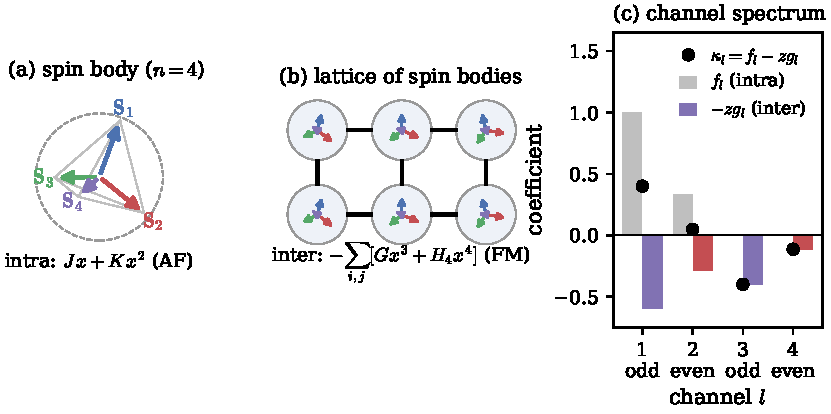
\includegraphics[width=\textwidth]{fig/fig_model.pdf}
\caption{Model. (a) A spin body of $n=4$ spins. Intra-body AF exchange $Jx+Kx^2$ ($x=\Sv_i\cdot\Sv_j$) favors the regular tetrahedron. (b) Bodies on a lattice are coupled by $-\sum_{i,j}[G x^3+H_4 x^4]$ between \emph{all} pairs of spins of neighboring bodies, so the coupling cannot tell which spin is which. (c) Channel spectrum for $J=1$, $K=0.5$, $zG=1$, $zH_4=0.5$: intra coefficients $f_l$, inter coefficients $-zg_l$, and their sum $\kappa_l$. Odd channels ($l=1,3$) carry magnetization; even channels ($l=2,4$) carry nematic order.}
\label{fig:model}
\end{figure*}

%=====================================================================
\section{Model and multipole channels}\label{sec:model}
%=====================================================================

Each site $a$ of a lattice with coordination $z$ hosts a body of $n$ unit vectors $\Sv_{a,i}$. The Hamiltonian is
\begin{align}
H&=\sum_a\sum_{i<j}\big[Jx^{aa}_{ij}+K(x^{aa}_{ij})^2\big]\nonumber\\
&\quad-\sum_{\langle ab\rangle}\sum_{i,j=1}^{n}\big[G(x^{ab}_{ij})^3+H_4(x^{ab}_{ij})^4\big],
\label{eq:H}
\end{align}
with $x^{ab}_{ij}=\Sv_{a,i}\cdot\Sv_{b,j}$ and $J=1$. The inter-body sum runs over all $n^2$ pairs, so $H$ is invariant under independent permutations $S_n$ of the spins of each body. We use the square ($z=4$) and simple cubic ($z=6$) lattices and quote couplings as $zG$ and $zH_4$.

\paragraph*{Channel decomposition.} Expanding a pair function in Legendre polynomials, $f(x)=\sum_l f_lP_l(x)$, and using the addition theorem gives, for a uniform state,
\begin{align}
E_{\rm body}&=\frac12\sum_l\kappa_lA_l+{\rm const},\label{eq:channel}\\
A_l&=\sum_{i,j}P_l(\Sv_i\cdot\Sv_j)=\frac{4\pi}{2l+1}|\qv^{(l)}|^2,\nonumber
\end{align}
where $q^{(l)}_m=\sum_iY_{lm}(\Sv_i)$ is the body multipole and $\kappa_l=f_l-zg_l$. For Eq.~\eqref{eq:H},
\begin{align}
\kappa_1&=J-\tfrac35zG, & \kappa_2&=\tfrac23K-\tfrac47zH_4,\nonumber\\
\kappa_3&=-\tfrac25zG, & \kappa_4&=-\tfrac{8}{35}zH_4.
\label{eq:kappa}
\end{align}
A monomial $x^k$ has non-negative Legendre coefficients, so a ferromagnetic monomial coupling contributes $g_l\ge0$ in every channel it contains. Note that $x^3=(2P_3+3P_1)/5$: a ``cubic'' coupling also contains a dipole part.

\paragraph*{Uniform-state theorem.} If $g_l\ge0$ for all $l$, the zero-temperature ground state is uniform on any lattice. On each bond, $-g_l\qv_a\cdot\qv_b\ge-\tfrac{g_l}{2}(|\qv_a|^2+|\qv_b|^2)$, so the total energy is bounded below by a sum of single-body energies, and the bound is reached when all $\qv_a$ coincide. The problem therefore reduces exactly to $n$ particles on the unit sphere interacting through the pair potential
\begin{equation}
\Phi(x)=\sum_l\kappa_lP_l(x).
\label{eq:Phi}
\end{equation}
Positive $\kappa_l$ spreads the particles (spherical designs~\cite{Delsarte1977}), and negative $\kappa_l$ makes them merge, in direct analogy with the cluster criterion for bounded pair potentials~\cite{Likos2001}. Phases are therefore classified by the partition of $n$ into coincident spins and the geometry of the resulting directions.

%=====================================================================
\section{Zero-temperature phases and exact boundaries}\label{sec:T0}
%=====================================================================

Figure~\ref{fig:T0} shows the ground-state phases for $n=4$, obtained by minimizing Eq.~\eqref{eq:Phi} over all configurations, together with the analytic boundaries derived below. Five phases appear: the tetrahedron T ($M=0$, a two-design), a ferrimagnet U (a coincident pair plus two single spins at $120^\circ$, $|M|/n=1/4$ exactly), a bent pair of dimers D, the collinear nematic C ($\uparrow\uparrow\downarrow\downarrow$, $M=0$), and the ferromagnet F. Note that partially collapsed phases (U, D) have no counterpart in rigid-polyhedron models.

\begin{figure*}[t]
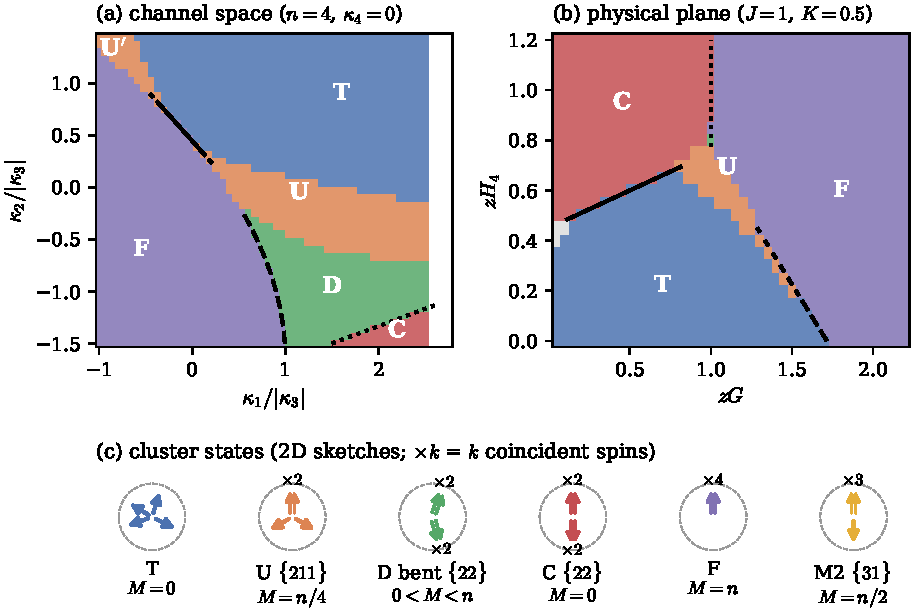
\includegraphics[width=\textwidth]{fig/fig_T0.pdf}
\caption{Zero-temperature phases for $n=4$. (a) Channel space with $\kappa_3=-1$, $\kappa_4=0$, from direct minimization (colors) and exact boundaries (black): T--F, Eq.~\eqref{eq:TF} (solid), D--F, Eq.~\eqref{eq:DF} (dashed), and C--D, Eq.~\eqref{eq:CD} (dotted). U$^\prime$ is an umbrella variant of U. (b) Physical plane at $J=1$, $K=0.5$ with T--C (solid), T--F (dashed), and C--F (dotted) boundaries of Table~\ref{tab:phases}. (c) Sketches of the cluster states; $\times k$ marks $k$ coincident spins.}
\label{fig:T0}
\end{figure*}

\paragraph*{Ferro--nematic theorem.} The F and C states both reach the maximum $A_l=n^2$ in every even channel. In odd channels F has $A_l=n^2$ while C has $A_l=M^2=0$. Hence
\begin{equation}
E_F-E_C=\frac{n^2}{2}\sum_{l\,{\rm odd}}\kappa_l\;\Rightarrow\;
z\,g_{\rm odd}(1)=f_{\rm odd}(1),
\label{eq:CF}
\end{equation}
with $h_{\rm odd}(1)=[h(1)-h(-1)]/2$. For Eq.~\eqref{eq:H} this is $zG=J$, independent of $K$, $H_4$, and $n$. Odd channels can therefore only drive collapse into ferromagnetism, and even channels only into the collinear nematic.

\paragraph*{Other boundaries.} With the closed-form energies of Table~\ref{tab:phases}, T--F and T--C are
\begin{equation}
\kappa_1+\kappa_2=-\tfrac49\kappa_3-\tfrac{20}{27}\kappa_4,\qquad
\kappa_2=\tfrac59\kappa_3-\tfrac{20}{27}\kappa_4.
\label{eq:TF}
\end{equation}
In physical units these read $(7/9)zG+(20/27)zH_4=J+2K/3$ and $zH_4=0.9K+0.3zG$. The D phase is a pair of dimers at angle $c=\cos\theta$, with energy $4\Phi(1)+4\Phi(c)$. It bends continuously out of C when $\Phi'(-1)$ changes sign,
\begin{equation}
\kappa_1-3\kappa_2+6\kappa_3-10\kappa_4=0\;\Leftrightarrow\;zG=\frac{J-2K+4zH_4}{3},
\label{eq:CD}
\end{equation}
and meets F first-order at
\begin{equation}
\kappa_1+\tfrac34\kappa_2+\tfrac38\kappa_3-\frac{9\kappa_2^2}{40\kappa_3}=0\quad(\kappa_4=0).
\label{eq:DF}
\end{equation}
All boundaries agree with the numerical minimization to the grid resolution [Fig.~\ref{fig:T0}] and with the low-temperature Monte Carlo phases.

\paragraph*{Local stability.} The Hessian of the tetrahedron splits under $T_d$ into three rotational zero modes and $E$ and $T_2$ modes with
\begin{align}
\lambda_{T_2}&=\tfrac83(\kappa_1+\kappa_2)-\tfrac{32}{3}\kappa_3+\tfrac{160}{81}\kappa_4,\nonumber\\
\lambda_E&=8\kappa_2-\tfrac{40}{3}\kappa_3-\tfrac{40}{9}\kappa_4.
\end{align}
For pure cubic inter-body coupling both eigenvalues \emph{increase} with $G$, because the tetrahedron is a local maximum of the octupole $A_3$. The T phase therefore never becomes locally unstable, and its collapse is nucleation driven. The F state is locally stable when $\Phi'(1)=\sum_l\kappa_l\,l(l+1)/2<0$.

\begin{table*}[t]
\caption{Phases of the $n=4$ model: isotropy group $H\subset O(3)$ (time reversal acts as inversion), fundamental group of the order-parameter space, non-zero multipoles, and zero-temperature energy per body for $L=0$, $G_1=0$ in Eq.~\eqref{eq:H}.}
\label{tab:phases}
\begin{ruledtabular}
\begin{tabular}{lllll}
Phase & $H$ & $\pi_1$ & $\qv^{(l)}\neq0$ & $E_{\rm body}$\\
\hline
T & $T_d$ & $2T$ & $l=3,4$ & $-2J+\tfrac23K-z(\tfrac{16}{9}G+\tfrac{56}{27}H_4)$\\
U, D & $C_{2v}$ & $\mathbb{Z}_4$ & all & numerical\\
C & $D_{\infty h}$ & $\mathbb{Z}_2$ & $l=2,4$ & $-2J+6K-8zH_4$\\
F & $C_{\infty v}$ & $0$ & all & $6J+6K-8z(G+H_4)$\\
\end{tabular}
\end{ruledtabular}
\end{table*}

%=====================================================================
\section{Symmetry, topology, and Landau invariants}\label{sec:sym}
%=====================================================================

\paragraph*{Full symmetry and chirality.} Every term of Eq.~\eqref{eq:H} depends only on dot products, so $H$ is invariant under $O(3)=SO(3)\times\{1,-1\}$, where $-1$ is time reversal. All isotropy groups in Table~\ref{tab:phases} contain improper elements. For example, time reversal maps a tetrahedron onto its dual, which is a $90^\circ$ rotation of the original. Hence $\pi_0=0$: there are no chiral domains and no vestigial chiral phase of the type found for chiral polyhedral nematics~\cite{Liu2016}. The allowed vestigial phases follow from the group chains $T_d\subset O_h$ (a cubatic phase with only $l=4$ order) and $C_{\infty v}\subset D_{\infty h}$ (a nematic phase left behind by a melting ferromagnet).

\paragraph*{Landau invariants.} The number of rotational invariants of a multipole order parameter $\qv^{(l)}$ follows from the character formula. Cubic invariants exist only for even $l$, because $(l\,l\,l;0\,0\,0)$ vanishes for odd $l$ (Table~\ref{tab:landau}). The nematic ($l=2$) and cubatic ($l=4$) transitions out of the isotropic phase are therefore first order in mean-field theory, whereas for the tetrahedral octupole ($l=3$) Landau theory does \emph{not} enforce a first-order transition [Fig.~\ref{fig:landau}]. A first-order transition can still arise through the coupling $(3\,3\,4)$ to the induced hexadecapole, or through fluctuations. The two independent quartic invariants of $l=3$ select between the two most symmetric octupole orbits, $T_d$ ($xyz$) and $D_{3h}$ ($\mathrm{Re}(x+iy)^3$). These are exactly the octupoles of the $n=4$ tetrahedron and of the $n=6$ prism (Sec.~\ref{sec:n6}), so both cluster sizes are two branches of a single octupolar Landau theory.

\begin{table}[b]
\caption{Number of independent rotational invariants of $\qv^{(l)}$.}
\label{tab:landau}
\begin{ruledtabular}
\begin{tabular}{lccccc}
$l$ & 1 & 2 & 3 & 4 & 6\\
\hline
cubic & 0 & 1 & 0 & 1 & 1\\
quartic & 1 & 1 & 2 & 2 & 3\\
\end{tabular}
\end{ruledtabular}
\end{table}

\begin{figure*}[t]
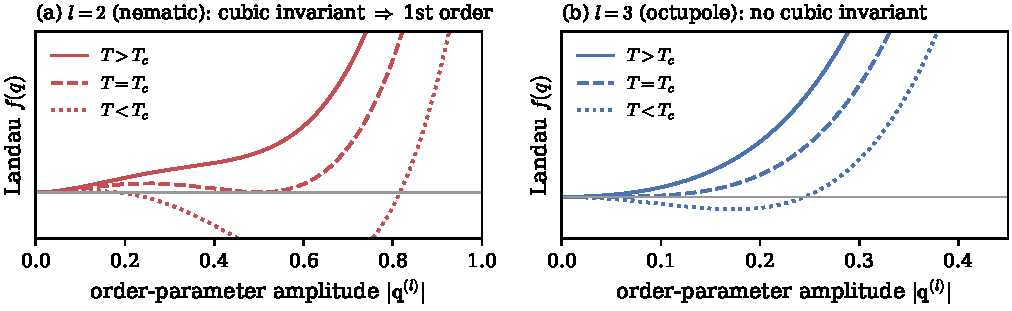
\includegraphics[width=\textwidth]{fig/fig_landau.pdf}
\caption{Landau free energies. (a) With a cubic invariant ($l=2$), a second minimum appears at finite amplitude and the transition is first order. (b) Without one ($l=3$), the minimum moves continuously away from zero. In the full theory the induced $l=4$ component can still make the $l=3$ transition weakly first order.}
\label{fig:landau}
\end{figure*}

\paragraph*{Defect algebra of the T phase.} Lifting $T$ to $SU(2)$ gives the binary tetrahedral group $2T$ of order 24 with seven conjugacy classes. Line defects (or point defects in 2D) are labeled by these classes. In an isotropic-stiffness approximation their energy scales with the square of the rotation angle [Fig.~\ref{fig:defects}]. The $2\pi$ class and the $4\pi/3$ classes are unstable to splitting, so the elementary defects are the eight $2\pi/3$ elements. Non-commuting lines cannot cross freely~\cite{PoenaruToulouse1977,Mermin1979}. For example, the $\pi$ lines about $x$ and $y$ leave a connecting rung with holonomy $[i,j]=-1$. On a periodic lattice the ordered product of plaquette holonomies equals the commutator of the two winding holonomies, so a single non-trivial defect is allowed on a torus. In the Abelian phases U, D ($\mathbb{Z}_4$) and C ($\mathbb{Z}_2$) lines cross freely.

\begin{figure}[tb]
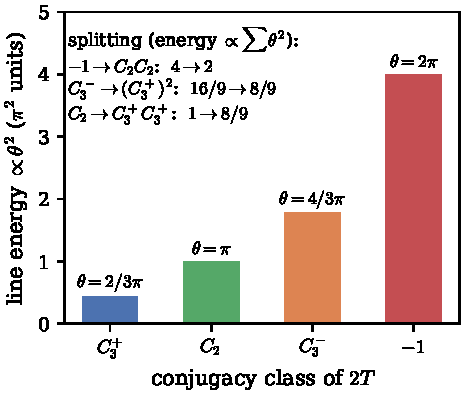
\includegraphics[width=\columnwidth]{fig/fig_defects.pdf}
\caption{Defect classes of the T phase, labeled by their rotation angle $\theta$, with line energy $\propto\theta^2$ (isotropic-stiffness estimate). The box lists the energetically favored splittings; the $C_2$ splitting is marginal and depends on elastic anisotropy.}
\label{fig:defects}
\end{figure}

%=====================================================================
\section{Entropic selection near the ferro--nematic line}\label{sec:entropy}
%=====================================================================

At $zG=J$ the C and F states are degenerate [Eq.~\eqref{eq:CF}], and so is every collinear state with $k$ reversed spins and moment $M=n-2k$. Near this line their energies are exactly
\begin{equation}
E_k-E_F=\tfrac12 x\,(n^2-M^2),\qquad x=zG-J,
\end{equation}
which is concave in $M$. Two entropic contributions distinguish them. The first is the harmonic spin-wave free energy $\tfrac{T}{2}\sum_{\mathbf q}\ln\det{}'\mathcal{H}(\mathbf q)$ of the uniform state, with global zero modes removed. The second is a configurational term $-T\ln\binom{n}{k}$, which counts the labelings of which spins are reversed. It is exact because the inter-body coupling fixes only $M_a$, not the labels, and it is convex in $M$. Defining $u=x/T$,
\begin{align}
\frac{\Delta F_k}{T}&=a_ku+\delta_k,\qquad a_k=\frac{n^2-M^2}{2},\label{eq:ladder}\\
\delta_k&=\tfrac12\ln\frac{\det{}'_k}{\det{}'_F}-\ln\binom{n}{k}.\nonumber
\end{align}
The equilibrium state is the lower envelope of these straight lines [Fig.~\ref{fig:ladder}]. For $n=4$ this envelope contains an intermediate collinear ferrimagnet M2 ($\uparrow\uparrow\uparrow\downarrow$) whenever $4\delta_{\rm M2}<3\delta_C$, which holds. The predicted phase sequence on heating at fixed $zG>J$ is therefore F$\to$M2$\to$C: a \emph{reentrant} nematic phase stabilized by entropy, with the ferromagnet at low temperature.

\begin{figure}[tb]
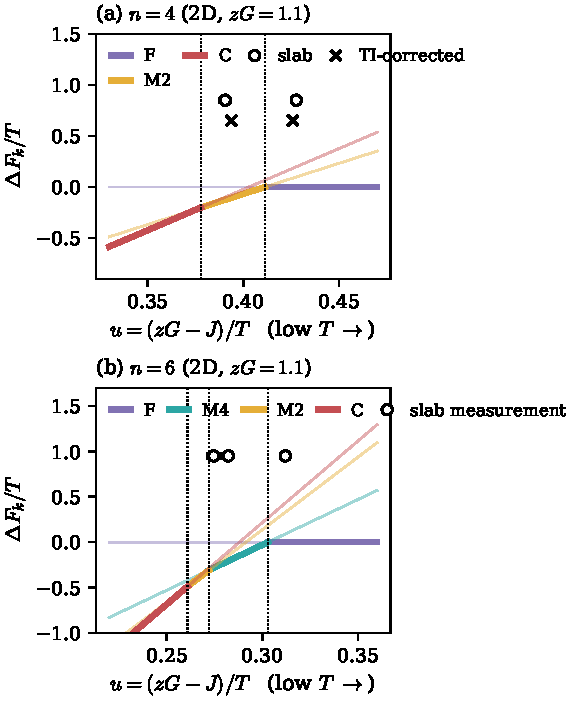
\includegraphics[width=\columnwidth]{fig/fig_ladder.pdf}
\caption{Entropic ladder, Eq.~\eqref{eq:ladder}, for the 2D model at $zG=1.1$. Thick segments mark the lower envelope (equilibrium phase); dotted lines are phase boundaries. (a) $n=4$: F$\to$M2$\to$C, boundaries at $u=0.411$ and $0.378$. (b) $n=6$: F$\to$M4$\to$M2$\to$C at $u=0.303$, $0.272$, $0.261$. Open circles on top: boundaries measured by slab coexistence, $u=(zG-J)/T$ ($n=6$: M4 resolved, M2 not); crosses in (a): thermodynamic-integration prediction.}
\label{fig:ladder}
\end{figure}

The theory gives three parameter-free predictions for the 2D model at $K=0.5$, $zH_4=1.5$, which we tested:
(1)~The low-temperature slope of the boundary, $zG^*(T)=J+aT+bT^2$. Harmonic plus label theory gives $a=0.382$ for a direct C$|$F boundary and $a=0.390$ for the F$|$M2 boundary. The label term alone gives $0.224$, and the harmonic term alone gives $0.158$.
(2)~A reentrance temperature $T_{\rm re}\simeq0.234\pm0.008$ at $zG=1.1$, obtained from the low-temperature fit.
(3)~A wedge of M2 between $T_1=0.2431$ and $T_2=0.2646$ at $zG=1.1$ (2D), and between 0.2440 and 0.2665 in 3D.

\paragraph*{Anharmonic correction.} Higher orders enter through the measured anharmonic energy of each branch, $\delta e(T)=e(T)-e_0-\tfrac{n_{\rm dof}}{2}T$. The Gibbs--Helmholtz relation gives
\begin{equation}
\delta f(T)=-T\int_0^T\frac{\delta e(T')}{T'^2}\,dT',
\label{eq:TI}
\end{equation}
which reduces to $-cT^2$ when $\delta e=cT^2$ but needs no polynomial fit.

%=====================================================================
\section{Monte Carlo method and decision rules}\label{sec:MC}
%=====================================================================

We simulate Eq.~\eqref{eq:H} with single-spin Metropolis moves, rigid rotations of whole bodies, and merge/split moves that propose a spin near another spin of the same body. The merge/split proposal density is a von Mises--Fisher mixture, included exactly in the acceptance ratio and verified by mutation tests. Parallel tempering~\cite{Hukushima1996} is used across continuous and weakly first-order transitions. Strongly first-order points are bracketed by separate heating and cooling ladders, and their transition temperatures are fixed by direct slab coexistence~\cite{Espinosa2013}: two phases share an interface and the sign of the interface velocity is recorded. Equilibrium boundaries near the ferro--nematic line come from slab coexistence and from the Clausius--Clapeyron slope
\begin{equation}
\frac{dzG^*}{dT}=\frac{\Delta E/T}{\langle\partial_{zG}H\rangle_C-\langle\partial_{zG}H\rangle_F},
\end{equation}
measured in single-phase chains. Order parameters are the uniform multipole moments $m_l=|\sum_a\qv_a^{(l)}|/(Nn)$, which are invariant under spin relabeling. First-order character is judged from energy histograms with an autocorrelation-corrected BIC~\cite{ChallaLandauBinder1986}, the Binder-type energy cumulant $V$, and the size dependence of the specific-heat maximum, $C_{\max}\propto N^{a}$. Defects are detected from plaquette holonomies in $2T$, obtained by Kabsch alignment~\cite{Kabsch1976} of each body to the tetrahedron, both on single bodies and on coarse-grained octupole moments. Lattice sizes are $L=16$--32 in 2D and $L=8$--16 in 3D.

All hypotheses H1--H12 were stated, with numerical decision rules, before the corresponding production runs. Where a rule or an estimator later proved inadequate we kept the original verdict, dated the change in the repository, and report the sequence here. Three changes were made after data had been seen. (i)~The slab zero-crossing estimator for the boundary slope was changed twice after the first temperature ($T=0.10$) had been analyzed: from a global linear fit to separate fits on the two sides of the zero, then with seed resampling and a window-choice systematic. The $T=0.10$ point is therefore not an independent test; the other four temperatures were analyzed after the estimator was fixed, and six alternative estimators change the slope by at most $0.008$ (Sec.~\ref{sec:results}\,B). (ii)~After the 2D wedge measurement, the primary zero-crossing error was changed from the bootstrap standard deviation, which was inflated by rare extrapolated resamples, to the half-width of the 16--84\% interval; the change applies only to later measurements. (iii)~For the 3D wedge, the pre-registered estimator reverted to first-sign-change interpolation in noisy bins and failed its rule. A seed-averaged estimator was then fixed, $T_2$ was remeasured with it, and the earlier $T_1$ data were recomputed; the latter is not an independent test. The failed verdicts remain in the record. The anharmonic correction was done first with a polynomial fit of the branch energies and then, with a rule fixed beforehand, by thermodynamic integration; both are reported. Table~\ref{tab:verdicts} lists the outcomes.

\begin{table}[tb]
\caption{Pre-registered hypotheses and verdicts. ``Rule'' is the verdict of the rule fixed before the run; supplementary measurements are listed separately.}
\label{tab:verdicts}
\begin{ruledtabular}
\begin{tabular}{p{0.34\columnwidth}p{0.6\columnwidth}}
Hypothesis & Verdict (key numbers)\\
\hline
H1 octupolar T transition (3D) & consistent with continuous, $zG=0.5,1,1.5$; $a(12\!\to\!14)=0.14$\\
H2 defect unbinding (2D) & undecidable (detector resolution)\\
H3 nematic C, 3D & first order; $T_c=0.356(2)$, latent heat $2.05(3)$\\
H5 ferrimagnet U & supported (2D, 3D); $m_1=0.24$--$0.25$\\
H6 boundary slope & harmonic+label supported; $a=0.392(10)$\\
H7 vestigial nematic & two separated transitions (4 points)\\
H12 C$\to$D & consistent with continuous (4 points)\\
Reentrance F$\to$C & rule: seen on heating only (rule design error); slab: $T_{\rm re}=0.2300(26)$\\
M2 wedge 2D/3D & located; final rule (3D): confirmed (width $0.0185$ vs $2\sigma=0.0129$)\\
Anharmonic (TI) & wedge positions within $0.3$--$1.2\sigma$ (Table~\ref{tab:TI}); $b$ at the $2\sigma$ edge\\
ladder $n=6$ (2D) & M4 phase confirmed; M2 not resolved (gap $0.0098$ vs $2\sigma=0.0099$)\\
\end{tabular}
\end{ruledtabular}
\end{table}

%=====================================================================
\section{Results}\label{sec:results}
%=====================================================================

\subsection{Channel selection at finite temperature}

The theorem of Eq.~\eqref{eq:CF} has a direct finite-temperature consequence: an order that lives only in even channels is insensitive to the odd-channel coupling $G$. Figure~\ref{fig:channel} shows three tests. First, along cut E ($K=-0.5$, $zH_4=0$) the inter-body coupling is purely odd, and collinear C bodies, which have $A_{\rm odd}=0$, do not couple at all; no nematic transition is found. Second, along cut E$^\prime$ ($K=-0.25$, $zH_4=0.25$) the nematic temperature ($T_2=0.240$--$0.242$ in 2D, $0.254$ in 3D, for all sizes) is the same at $zG=0.9$ and $1.0$, while the magnetization of the D phase orders at $T_1=0.094$ and $0.18$ in 2D ($0.104$ and $0.190$ in 3D), respectively. Third, along cut D ($zH_4=1.5$), $T_2=0.618$--$0.623$ is again independent of $zG$. Because the D phase couples only through odd channels, its ordering temperature scales as $G\,M^2$, with $M^2\propto zG-zG_c$ near the C--D boundary of Eq.~\eqref{eq:CD}. This estimate gives the correct trend in both cuts (ratio $T_1(zG{=}1)/T_1(zG{=}0.9)$: 2.8 predicted, 1.90 measured in 2D and 1.82 in 3D for E$^\prime$; $T_1(0.8)/T_1(1.0)$: 0.32 predicted, 0.28 measured for E, from a preliminary $L=8$ trial). In 3D, $T_1$ and $T_2$ remain separated as $L$ grows (H7), giving a vestigial nematic between the D and isotropic phases. The C$\to$D transition is consistent with being continuous (H12), as expected for a vector order parameter $\mathbf M_\perp$ without a cubic invariant.

\begin{figure*}[t]
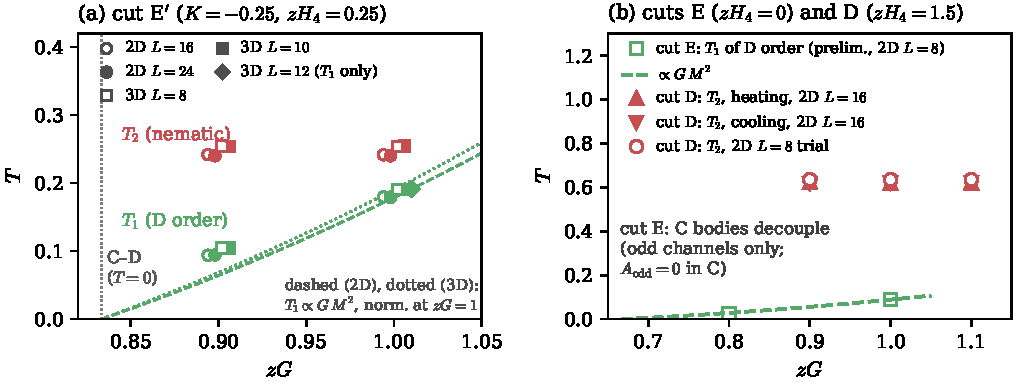
\includegraphics[width=\textwidth]{fig/fig_channel.pdf}
\caption{Channel selection at finite temperature, from the individual runs. (a) Cut E$^\prime$: the nematic temperature $T_2$ (red) does not depend on the odd-channel coupling $zG$, while the D-phase ordering temperature $T_1$ (green) does. Circles: 2D, $L=16$ (open) and $24$ (filled); squares: 3D, $L=8$ (open) and $10$ (filled); diamonds: 3D $L=12$, where the ladder (0.8--1.2\,$T_1$) does not reach $T_2$. Error bars are jackknife errors of the susceptibility peaks. Dashed (2D) and dotted (3D) lines: $T_1\propto G M^2$ normalized at $zG=1$. (b) Cut E: $T_1$ of the D order in a preliminary $L=8$ trial with ordered start (squares) and the same scaling; the C state at $zG=0.5$ shows no order. Cut D: $T_2$ from the specific-heat peak of heating and cooling ladders ($L=16$, triangles) and an $L=8$ trial (circles).}
\label{fig:channel}
\end{figure*}

\subsection{Entropic selection, reentrance, and the M2 wedge}

Figure~\ref{fig:H6} collects the results near the ferro--nematic line. Slab coexistence at $T=0.10$--$0.20$ gives $a=0.392\pm0.010$ and $b=0.15\pm0.05$ (2D). This value excludes the label-only (0.224) and harmonic-only (0.158) predictions by more than $12\sigma$ and agrees with the harmonic plus label value. As the M2 wedge shows, the measured boundary is in fact the F$|$M2 line, whose prediction 0.390 coincides with an auxiliary rescan, $0.390\pm0.007$. Sensitivity tests over six zero-crossing estimators give $a=0.384$--$0.392$, all with the same verdict. Figure~\ref{fig:H6} shows the individual zero crossings; the first $T=0.175$ and $0.20$ zeros lie at the edge of the scanned range and are replaced there by the values of a rescan with a larger range.

At $zG=1.1$ the ferromagnet re-enters the nematic on heating. Because the boundary is strongly first order, heating ladders superheat F to $T=0.316$ and cooling ladders never leave C. The pre-registered rule, which required both ladders, therefore could not be met. Direct coexistence gives the equilibrium $T_{\rm re}=0.2300\pm0.0026$, inside the predicted window and consistent with the extrapolated fit $0.234\pm0.008$.

The M2 wedge was predicted before it was measured. In 2D, slab coexistence of F$|$M2 and M2$|$C gives $T_1=0.2338\pm0.0005$ and $T_2=0.2560\pm0.0019$. In 3D ($L=12$), the final rule with a seed-averaged estimator gives $T_1=0.2356\pm0.0008$ and $T_2=0.2541\pm0.0064$, a width of $0.0185$ that exceeds twice its uncertainty. An earlier 3D estimator failed on this criterion because it reverted to first-sign-change interpolation; that verdict is retained in the record.

Both positions lie about $0.01$ below the harmonic prediction, with the same sign in 2D and 3D. Including the anharmonic free energy by thermodynamic integration, Eq.~\eqref{eq:TI}, of the measured branch energies moves all four wedge temperatures onto the measurements (Table~\ref{tab:TI}); the corrected values differ from the measurements by $0.3$--$1.2$ combined standard deviations (by $2.0$, $1.1$, $0.5$, and $0.3$ times the measurement error alone). The curvature $b$ is reproduced only at the $2\sigma$ edge ($0.054(4)$ versus $0.15(5)$); its prediction error is negligible, so this test is limited by the measurement. The integral uses branch energies from $T=0.02$ to $0.26$ on $16^2$ (2D) and $8^3$ (3D) lattices, which are smaller than the slabs. A polynomial fit of the same energies gives the same direction, but its prediction error ($0.017$--$0.06$) is dominated by the choice of fit range, which is why we use the integral.

\begin{table}[tb]
\caption{Thermodynamic-integration (TI) prediction against slab measurement at $zG=1.1$ (2D $L=24$ slab, 3D $L=12$ slab; branch chains $16^2$ and $8^3$). The prediction error is the propagated statistical error of the branch energies; $\Delta/\sigma$ divides the difference by the combined error. $T_1$: F$\to$M2, $T_2$: M2$\to$C; $b$ is the curvature of the 2D boundary $zG^*=J+aT+bT^2$.}
\label{tab:TI}
\begin{ruledtabular}
\begin{tabular}{lcccc}
 & harmonic & TI & measured & $\Delta/\sigma$\\
\hline
$T_1$ (2D) & 0.2431 & 0.2348(7) & 0.2338(5) & 1.2\\
$T_2$ (2D) & 0.2646 & 0.2539(23) & 0.2560(19) & 0.7\\
$T_1$ (3D) & 0.2440 & 0.2352(5) & 0.2356(8) & 0.4\\
$T_2$ (3D) & 0.2665 & 0.2560(18) & 0.2541(64) & 0.3\\
$b$ (2D) & 0 & 0.054(4) & 0.15(5) & 1.9\\
\end{tabular}
\end{ruledtabular}
\end{table}

\begin{figure}[tb]
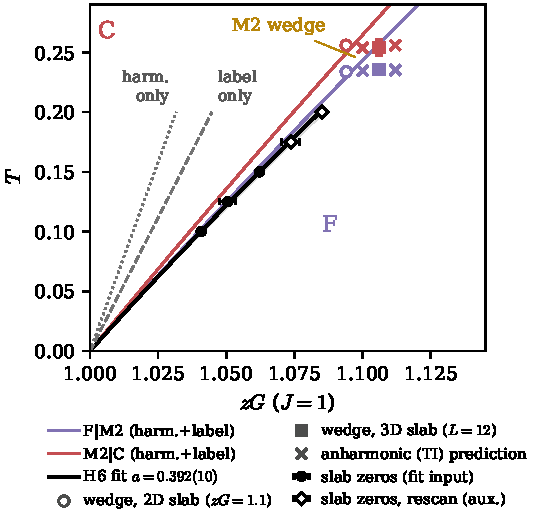
\includegraphics[width=\columnwidth]{fig/fig_H6.pdf}
\caption{Phases near the ferro--nematic line (2D, $K=0.5$, $zH_4=1.5$). Thin colored lines: harmonic plus label predictions for F$|$M2 and M2$|$C. Black line and band: fit $zG^*=1+aT+bT^2$; black symbols: the individual slab zero crossings (dots: input to the fit; open diamonds: rescan of $T=0.175$ and $0.20$ with a larger range, auxiliary). Gray lines: label-only and harmonic-only slopes. At $zG=1.1$: wedge boundaries $T_1$ (F$|$M2, purple) and $T_2$ (M2$|$C, red) from slab coexistence in 2D (open circles) and 3D (squares) with their errors, and the thermodynamic-integration predictions ($\times$).}
\label{fig:H6}
\end{figure}

\subsection{Transition order}

Figure~\ref{fig:order} compares the effective exponent $a=d\ln C_{\max}/d\ln N$ across transitions. For the octupolar transition of the T phase (cut A), the exponents between the two largest sizes are $0.14(24)$ at $zG=0.5$ ($L=12\to14$), $0.22(18)$ at $1.0$, and $0.17(11)$ at $1.5$ (Fig.~\ref{fig:order}a), energy histograms are unimodal, and $|2/3-V_{\min}|$ decreases with $L$. In 2D, the same exponent is consistent with zero ($-0.14$ for $L=24\to32$ at $zG=1$). We therefore classify this transition as consistent with continuous. At $zG=0.5$ the global fit over $L=8$--14 gives $a=0.48$ (68\% interval $0.42$--$0.53$), larger than any standard 3D universality class, although the pairwise values fall from $0.49$ and $0.67$ for the smaller pairs to $0.14(24)$ for $12\to14$. This leaves room for weak first-order behavior with a correlation length exceeding $L$, or for crossover near a tricritical point; an exploratory point at $zG=0.3$ did not support the latter. Transitions with an $l=2$ invariant are clearly first order. In 3D at $zH_4=1$, branch energies and the coexistence window are independent of $L$, with latent heat $2.05\pm0.03$ per body, while the slab-coexistence $T_c$ decreases from $0.3578(3)$ at $L=12$ to $0.3554(2)$ at $L=16$ (Fig.~\ref{fig:order}b). In 2D at $zH_4=2$ the specific-heat maximum grows with exponent $0.72(16)$ ($L=16\to24$). The contrast between $l=3$ and $l=2$ follows the Landau counting of Table~\ref{tab:landau}. It also distinguishes deformable spin bodies from rigid polyhedral gauge models, for which first-order transitions are generic~\cite{Liu2017}.

\begin{figure}[tb]
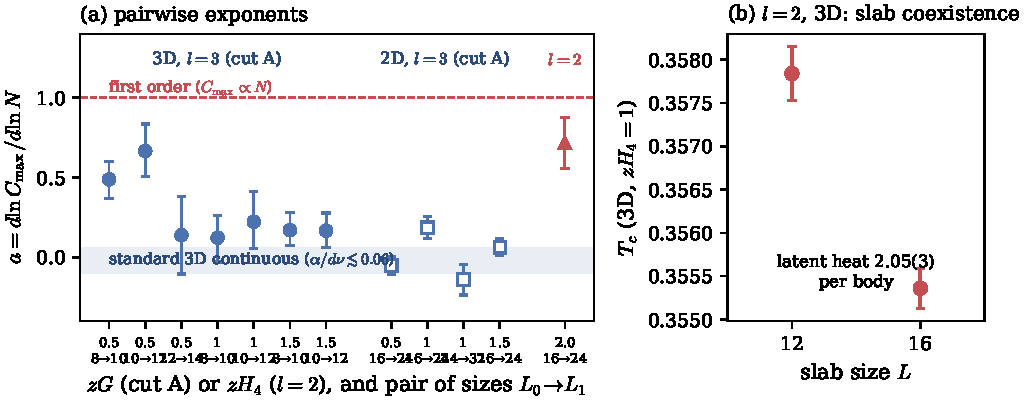
\includegraphics[width=\columnwidth]{fig/fig_order.pdf}
\caption{(a) Effective specific-heat exponent $a=d\ln C_{\max}/d\ln N$ for every pair of sizes $L_0\to L_1$, with 16--84\% errors from the block-jackknife errors of $C_{\max}$: the octupolar ($l=3$) transition of the tetrahedral phase in 3D (filled circles) and 2D (open squares), and the 2D nematic ($l=2$) transition at $zH_4=2$ (triangle). The band marks standard 3D continuous transitions and the dashed line first-order scaling. (b) $T_c$ of the first-order 3D nematic transition ($zH_4=1$) from slab coexistence at two slab sizes; the latent heat is from window chains.}
\label{fig:order}
\end{figure}

\subsection{Partially collapsed ferrimagnet}

The U phase, a dimer plus two single spins with $|M|/n=1/4$, is found at finite temperature in both 2D and 3D (cut C: $K=0$, $zH_4=0$, $zG=1.0$ and $1.2$). The measured magnetization $m_1=0.24$--$0.25$ matches the exact value, and the fraction of bodies in the $\{211\}$ partition is 1.00 at low temperature. In 3D the upper end of the U interval (0.140/0.143 and 0.176/0.177 for $L=8/10$) does not drift with $L$. U is therefore a genuine thermodynamic phase, not a finite-size effect.

\subsection{Defects}

In 2D the octupole correlation function decays algebraically over the accessible sizes. Because the $SO(3)/T$ sigma model is asymptotically free~\cite{Polyakov1975}, we interpret this as a crossover with a correlation length that grows like $\exp(c/T)$, not as quasi-long-range order. Defects of the $2T$ classes are detected reliably at low temperature. Near the crossover, however, the frame of individual bodies becomes ill defined before defects proliferate, and a scale-ratio test of defect unbinding is undecidable at our resolution (H2). In 3D the frame and the defects disappear together at the first-order transitions, as expected.

%=====================================================================
\section{Predictions for six-spin bodies}\label{sec:n6}
%=====================================================================

For $n=6$ the intra-body exchange selects a two-design. Among six points these form a continuous family: two triangles at height $\pm1/\sqrt3$, twisted by $\varphi$, interpolating between the prism P ($\varphi=0$, $D_{3h}$) and the octahedron O ($\varphi=60^\circ$, $O_h$). Along this family
\begin{equation}
A_3=\tfrac{10}{3}(1+\cos3\varphi),\qquad A_4=\tfrac{119}{9}-\tfrac{70}{9}\cos3\varphi,
\end{equation}
so the inter-body energy is linear in $\cos3\varphi$ with coefficient $\propto\tfrac43G-\tfrac{16}{9}H_4$ [Fig.~\ref{fig:n6}]. Cubic exchange selects the prism and quartic exchange selects the octahedron. On the line $zH_4=\tfrac34zG$ the entire family is degenerate. Because the octahedron has $A_3=0$, octahedral bodies couple only through $l=4$. Odd couplings instead favor dimerization into a planar triangle of dimers (``222'', $M=0$, $D_{3h}$), whose octupole $A_3/n^2=0.625$ exceeds that of any six-point design. Its boundaries with C and F are $zH_4=0.8K+0.4zG$ and $13.5zG+11.25zH_4=18J+9K$. The 222 phase shares the $D_{3h}$ symmetry of the prism, so the two can be connected continuously by flattening, and its defects form the non-Abelian group $\mathrm{Dic}_3$.

The entropic ladder of Eq.~\eqref{eq:ladder} for $n=6$ contains all four collinear states F$\to$M4$\to$M2$\to$C [Fig.~\ref{fig:ladder}(b)], with boundaries at $u=0.303$, $0.272$, and $0.261$ (2D, $zG=1.1$), that is $T=0.330$, $0.367$, and $0.383$. The ground-state competitors of this family are the four collinear states for $K=0.5$, $zH_4=1.5$ and $zG=0.95$--$1.2$; non-collinear states ($\{321\}$, $\{222\}$, $\{2211\}$) lie at least $4.8$ above. We tested the ladder by slab coexistence (2D, $L=24$, three seeds, interface pairs M4$|$F, M2$|$M4, C$|$M2). The three boundaries are at $T=0.3205(11)$, $0.3544(21)$, and $0.3641(45)$, i.e.\ $0.010$, $0.013$, and $0.019$ below the harmonic values, the same sign as for $n=4$ and growing with temperature. The M4 phase is resolved ($T_b-T_a=0.034$ against $2\sigma=0.005$); the M2 interval is not ($T_c-T_b=0.0098$ against $2\sigma=0.0099$). A refinement with six seeds on a finer grid did not help ($T_c=0.364(11)$): the C$|$M2 interface moves at less than $2\times10^{-4}$ per sweep, so longer runs are needed. The pre-registered verdict is therefore \emph{M4 confirmed, M2 not resolved}. The concave-energy versus convex-entropy mechanism generalizes to any $n$ and produces $\lfloor n/2\rfloor$ collinear steps when all of them lie on the lower envelope.

\begin{figure*}[t]
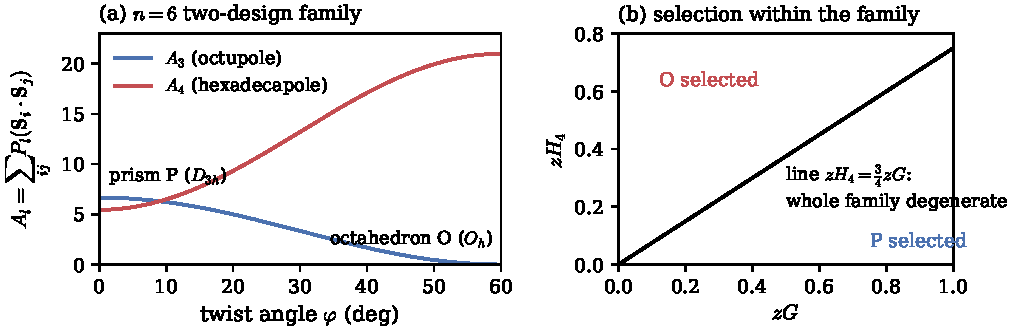
\includegraphics[width=\textwidth]{fig/fig_n6.pdf}
\caption{Six-spin bodies. (a) Octupole $A_3$ and hexadecapole $A_4$ along the two-design family from the prism to the octahedron. (b) Within this family the inter-body energy selects P or O; on the line $zH_4=\tfrac34zG$ the whole family is degenerate.}
\label{fig:n6}
\end{figure*}

%=====================================================================
\section{Discussion}\label{sec:disc}
%=====================================================================

\paragraph*{What is new.} Three features distinguish spin bodies from rigid polyhedra. First, couplings act channel by channel, and the parity of the channel decides whether a body can only magnetize or only align. This turns a many-parameter problem into a few exact inequalities [Eqs.~\eqref{eq:CF}--\eqref{eq:DF}]. Second, collapse produces phases with no rigid analog: partially merged ferrimagnets (U, D) and collinear states whose relative weights are set by a counting entropy. The resulting ladder is a simple and quantitative example of order by disorder~\cite{Villain1980,Henley1989} in which a discrete label entropy and the spin-wave entropy contribute comparably; both are needed to obtain the measured slope. Third, the transition order follows the Landau counting of invariants of the relevant multipole rather than a generic rule for polyhedral order.

\paragraph*{Where the model meets experiment.} The classical limit is natural when each ``spin'' is a mesoscopic moment, as in artificial spin systems and nanomagnet arrays~\cite{Heyderman2013,Skjaervo2020}. There, the dipolar interaction between elements contains exactly the multipole structure of Eq.~\eqref{eq:channel}, and clusters of elements can be engineered with strong internal coupling. For atomic spins the polyhedral picture requires large $S$. Exact diagonalization of a quantum four-spin body shows a clean rigid-rotor tower only for $S\gtrsim4$--6, and the permutation sector of the ground state depends on $2S \bmod 3$. This is a Berry-phase effect that we leave for future work. The cluster-multipole description of noncollinear antiferromagnets~\cite{Suzuki2017} and breathing pyrochlores~\cite{Okamoto2013,Rau2016} provides materials in which the channel selection rules may be tested directly.

\paragraph*{Limitations.} All analytic predictions rest on the uniform-state theorem (exact at $T=0$) and on low-temperature expansions. Size dependence was checked with two or three sizes, 3D wedge positions with one slab size, and the $n=6$ ladder with one size and three seeds; the anharmonic integral uses chains smaller than the slabs. The order of the octupolar transition at $zG=0.5$ remains open.

%=====================================================================
\section{Conclusion}
%=====================================================================

Bodies made of antiferromagnetically coupled spins behave as polyhedra only as long as the inter-body coupling respects their multipole content. Decomposing all couplings into Legendre channels gives a uniform-state theorem, exact phase boundaries, and a parity rule: odd channels magnetize and even channels align. At finite temperature, the competition between a concave collinear energy and a convex label entropy, together with spin-wave entropy, produces an entropic ladder. It accounts quantitatively for the boundary slope, a reentrant nematic phase, and an equilibrium collinear ferrimagnet, all confirmed by pre-registered simulations in two and three dimensions. Transitions with a cubic Landau invariant are first order, while the tetrahedral octupolar transition is consistent with continuous behavior, unlike rigid polyhedral models. The framework predicts a degenerate prism--octahedron family and a four-step ladder for six-spin bodies, and it provides a route to engineering non-Abelian orientational order from spins.

\begin{acknowledgments}
Simulation code, decision rules, the full record of verdicts, and the derived data tables behind every figure are available at https://github.com/cywon-commits/Polyhedron\_Spin\_Group (directory \texttt{paper/}).
\end{acknowledgments}

%=====================================================================
\appendix
\section{Harmonic free energy and label entropy}\label{app:harm}
%=====================================================================

For a uniform collinear state with $k$ reversed spins, the quadratic Hamiltonian in the $2nN$ transverse coordinates is block diagonal in $\mathbf q$. Its $2n\times2n$ blocks $\mathcal H_k(\mathbf q)$ are built from $\Phi'(\pm1)$ for intra-body pairs and $g'(\pm1)$ for inter-body pairs. The classical harmonic free energy is $F_k^{\rm harm}=\tfrac{T}{2}\sum_{\mathbf q}\ln\det{}'\mathcal H_k(\mathbf q)$, where the prime removes the global zero modes (two for collinear states). Each body independently chooses which $k$ of its $n$ spins are reversed, because uniformity is enforced only for $M_a$. This gives the exact configurational entropy $\ln\binom{n}{k}$ per body. Low-temperature energies satisfy $e(T)=e_0+\tfrac{n_{\rm dof}}{2}T(1-n_0/(2N))+O(T^2)$, with $n_0$ the number of global zero modes, which we verified to 1\%.

\begin{thebibliography}{99}
\bibitem{Fel1995} L. G. Fel, Phys. Rev. E \textbf{52}, 702 (1995).
\bibitem{Lubensky2002} T. C. Lubensky and L. Radzihovsky, Phys. Rev. E \textbf{66}, 031704 (2002).
\bibitem{SemenoffZhou2007} G. W. Semenoff and F. Zhou, Phys. Rev. Lett. \textbf{98}, 100401 (2007).
\bibitem{Kobayashi2009} M. Kobayashi, Y. Kawaguchi, M. Nitta, and M. Ueda, Phys. Rev. Lett. \textbf{103}, 115301 (2009).
\bibitem{KawaguchiUeda2012} Y. Kawaguchi and M. Ueda, Phys. Rep. \textbf{520}, 253 (2012).
\bibitem{Liu2016} K. Liu, J. Nissinen, R.-J. Slager, K. Wu, and J. Zaanen, Phys. Rev. X \textbf{6}, 041025 (2016).
\bibitem{Nissinen2016} J. Nissinen, K. Liu, R.-J. Slager, K. Wu, and J. Zaanen, Phys. Rev. E \textbf{94}, 022701 (2016).
\bibitem{Liu2017} K. Liu, J. Nissinen, J. de Boer, R.-J. Slager, and J. Zaanen, arXiv:1706.01811.
\bibitem{Suzuki2017} M.-T. Suzuki, T. Koretsune, M. Ochi, and R. Arita, Phys. Rev. B \textbf{95}, 094406 (2017).
\bibitem{Kuramoto2009} Y. Kuramoto, H. Kusunose, and A. Kiss, J. Phys. Soc. Jpn. \textbf{78}, 072001 (2009).
\bibitem{Okamoto2013} Y. Okamoto, G. J. Nilsen, J. P. Attfield, and Z. Hiroi, Phys. Rev. Lett. \textbf{110}, 097203 (2013).
\bibitem{Rau2016} J. G. Rau, L. S. Wu, A. F. May, L. Poudel, B. Winn, V. O. Garlea, A. Huq, P. Whitfield, A. E. Taylor, M. D. Lumsden, M. J. P. Gingras, and A. D. Christianson, Phys. Rev. Lett. \textbf{116}, 257204 (2016).
\bibitem{JamesKeenan1959} H. M. James and T. A. Keenan, J. Chem. Phys. \textbf{31}, 12 (1959).
\bibitem{Delsarte1977} P. Delsarte, J. M. Goethals, and J. J. Seidel, Geom. Dedicata \textbf{6}, 363 (1977).
\bibitem{Likos2001} C. N. Likos, A. Lang, M. Watzlawek, and H. L\"owen, Phys. Rev. E \textbf{63}, 031206 (2001).
\bibitem{PoenaruToulouse1977} V. Po\'enaru and G. Toulouse, J. Phys. (Paris) \textbf{38}, 887 (1977).
\bibitem{Mermin1979} N. D. Mermin, Rev. Mod. Phys. \textbf{51}, 591 (1979).
\bibitem{Hukushima1996} K. Hukushima and K. Nemoto, J. Phys. Soc. Jpn. \textbf{65}, 1604 (1996).
\bibitem{Espinosa2013} J. R. Espinosa, E. Sanz, C. Valeriani, and C. Vega, J. Chem. Phys. \textbf{139}, 144502 (2013).
\bibitem{ChallaLandauBinder1986} M. S. S. Challa, D. P. Landau, and K. Binder, Phys. Rev. B \textbf{34}, 1841 (1986).
\bibitem{Kabsch1976} W. Kabsch, Acta Crystallogr. A \textbf{32}, 922 (1976).
\bibitem{Polyakov1975} A. M. Polyakov, Phys. Lett. B \textbf{59}, 79 (1975).
\bibitem{Villain1980} J. Villain, R. Bidaux, J.-P. Carton, and R. Conte, J. Phys. (Paris) \textbf{41}, 1263 (1980).
\bibitem{Henley1989} C. L. Henley, Phys. Rev. Lett. \textbf{62}, 2056 (1989).
\bibitem{Heyderman2013} L. J. Heyderman and R. L. Stamps, J. Phys.: Condens. Matter \textbf{25}, 363201 (2013).
\bibitem{Skjaervo2020} S. H. Skj{\ae}rv{\o}, C. H. Marrows, R. L. Stamps, and L. J. Heyderman, Nat. Rev. Phys. \textbf{2}, 13 (2020).
\end{thebibliography}

\end{document}
